\chapter{Teori}\label{Teori}

\section{Brystets opbygning og brystkræft}
Bryster er sammensat af mange små brystkirtler, bestående af kirtelceller til producering af mælk, og udførselsgange, som samler sig frem til brystvorten. Det mandlige bryst er opbygget ligesom kvindebrystet, dog uden fungerende mælkekirtler \cite{Mand}. Brystkirtlerne er omgivet af fedt og bindevæv\cite{Bryst}.

\begin{figure}[H]
    \centering
    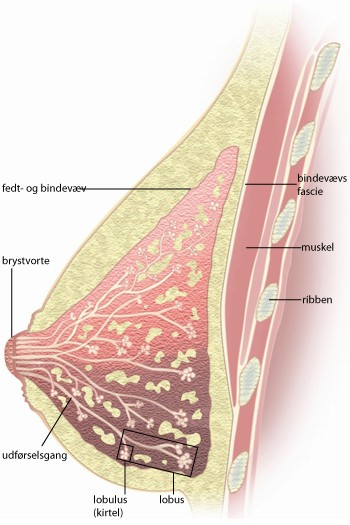
\includegraphics[width=0.35\textwidth]{figurer/r/bryst}
    \caption{Det kvindelige brystets opbygning \cite{Bryst}}
    \label{Brystet}
\end{figure}

I brystet kan der opstå brystkræft, hvor det hyppigst opstår i en udførselsgang \citep{Bryst}. Brystkræft er den mest udbredte kræftform hos kvinder, men det kan også opstå ved mænd. Det er dog meget hyppigere hos kvinder \cite{Mand}.

Forstadiet til brystkræften sker ved en mutation af cellernes gener. Denne mutation kan ske over tid, men kan det også være et arvet gen. Mutationen gør, at cellerne ændrer form og udseende, da cellerne deler sig for meget, hvilket danner en knude. Normalt vil syge celler nedbrydes, men dette sker ikke ved kræftceller, som hele tiden deler sig og skaber nye kræftceller. Bliver udviklingen af kræftcellerne ikke behandlet, vil kræftcellerne med tiden brede sig til det omkringliggende væv \cite{Udvikling}. 

\section{Ultralydsscanning}
Ultralyd er højfrekvent lyd, hvor man til ultralydsscanning benytter frekvenser mellem 2 og 20 MHz \cite{Frekvens}. Der anvendes en ultralydsprobe, som er en transducer. Transduceren indeholder piezoelektriske krystaller, som skaber lydbølger, når de bliver udsat for en elektrisk spænding. Disse lydbølger udsendes fra og reflekteres tilbage til transduceren, når de møder væv. Ud fra lydbølgerne, transduceren modtager, dannes en ultralydsscanning, som radiologen kan diagnosticere ud fra \cite{Ultralydsscanning}.

På ultralydsscanningen ses kirtelvæv som lyse områder, mens kræftknuder fremtræder som mørke skygger. Der er derfor en god kontrast mellem kirtelvæv og kræftknude på et ultralydsbillede \cite{Ultralyd}.

\section{Røntgenundersøgelse}
Røntgenstråler er elektromagnetiske bølger med en kortere bølgelængde end synligt lys. Strålerne er ioniserede, og derfor er det vigtigt at give den korrekte dosis, der måles med enheden milliSievert (mSv). Ved mammografiscanninger med røntgen benyttes en dosis på 0,5 mSv. \cite{Sundhedsstyrelsen}. Livstidsrisikoen for at inducere kræft efter en mammografiscanning med røntgen er definieret som meget lille, hvilket betyder, at 1 ud af 100.000 til 1 ud af 10.000 rammes, som følge af røntgenstråling \cite{Risk}. 

Ved røntgenundersøgelser sendes røntgenstrålerne fra et røntgenrør gennem patienten. De opfanges på en fotografisk film, som vil danne røntgenbilledet afhængig af, hvor meget af strålingen, der bliver absorberet i kroppen \cite{Rontgenundersogelse}.

På røntgenbilleder ses fedt og andre bløddele som grå skygger, da de ikke absorberer så mange røntgenstråler, hvorimod kræftknuder absorberer meget røntgenstråling og derfor ses som lyse områder \cite{Rontgenundersogelse}.
\newpage

På billedet \ref{rontgen} nedenfor ses et røntgenbillede af brystvæv. Kræftknuden ses tydeligt som den lysende plet, markeret med en firkant. Figur \ref{ultralyd} nedenfor viser øverst en teoretisk tegning af en ultralydscanning af brystvæv. Stilbilledet fra en ultralydsscanning af brystvæv, ses under tegningen. På billedet ses kræftknuden som en mørk skygge. 


\begin{figure}[H]
  \centering
  \begin{minipage}{0.4\textwidth}
    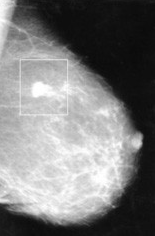
\includegraphics[width=\textwidth]{figurer/r/rontgen}
    \caption{Røntgenbillede \cite{Mammografi}}
    \label{rontgen}
  \end{minipage}
  \hfill
  \begin{minipage}{0.535\textwidth}
    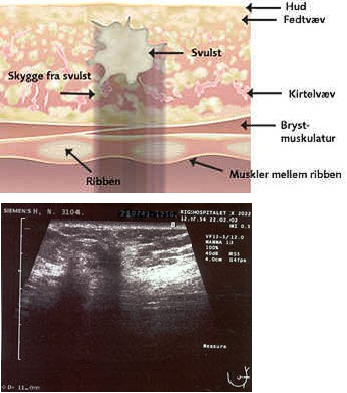
\includegraphics[width=\textwidth]{figurer/r/samlet}
    \caption{Tegning og ultralydsbillede \cite{Ultralyd}}
    \label{ultralyd}
  \end{minipage}
\end{figure}

